
\newpage

\section{Digital Filters}

\par \indentt With our DFT and IDFT matrices in hand, the process for digital filtering becomes clear: take a sample vector $\mathbf{x}$, apply the DFT to obtain a frequency vector $\lambda$, change the amplitudes of this vector, then apply the IDFT to obtain a new sample vector that generates the filtered sound. This leads us to the following definition for digital filters:

\begin{definition}
    A digital filter $S$ is diagonalizable to a diagonal matrix $D_{\lambda_S}$ whose diagonal terms are the terms of a frequency response vector $\lambda_S$. In other words, $S$ is a filter if  $$S=F^{-1}_ND_{\lambda_S}F_N \hspace{.5in} \text{for some } D_{\lambda_S} = \text{diag}(\lambda_S).$$
    \label{defn:digital_filter}
\end{definition}

\begin{figure}[h]
    \centering
    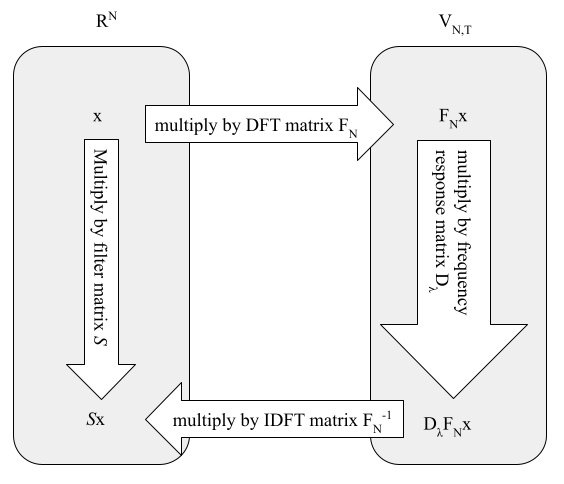
\includegraphics[scale=.5]{digital_filter_space_diagram.png}
    \caption{Moving within and between discrete time and the frequency space}
    \label{fig:digital_filter_space_diagram}
\end{figure}

\par \bigskip Once we use the DFT and IDFT to find $S$ for a desired frequency response, any sample vector $\mathbf{x}$ can be filtered to a new sample vector $S\mathbf{x}$.

\newpage

\begin{example}{The term in the $j$'th row and $k$'th column\footnote{For simplicity's sake, we will index filter matrices starting at 0 rather than 1 because the first row and column correspond to $n=0$ and $k=0$, respectively.} of a digital filter $S$ is given by}
    $$s_{j,k} = (F^{-1}_NDF_N)_{j,k} = (\frac{1}{\sqrt{N}})^2 \sum_{n=0}^{N-1} e^{-\frac{2\pi ikn}{N}} \lambda_S(\frac{n}{T}) \puretone{jn}{N} = \frac{1}{N} \sum_{n=0}^{N-1} \lambda_S(\frac{n}{T}) \puretone{(j-k)n}{N}.$$
    \label{ex:terms_digital_filter}
\end{example}

Note that:

$$s_{j+1,k+1} = \frac{1}{N} \sum_{n=0}^{N-1} \lambda_S(\frac{n}{T}) \puretone{(j+1-k-1)n}{N} = \frac{1}{N} \sum_{n=0}^{N-1} \lambda_S(\frac{n}{T}) \puretone{(j-k)n}{N} = s_{j,k}.$$

\par That means the entries of $S$ are equal along each diagonal. To put this another way, let $l = j-k$ and note that:

$$s_{\{l=j-k\}} = \frac{1}{N} \sum_{n=0}^{N-1} \lambda_S(\frac{n}{T}) \puretone{ln}{N}.$$

\par In other words, the entries of $S$ are equal to $\frac{1}{N} \sum_{n=0}^{N-1} \lambda_S(\frac{n}{T}) \puretone{ln}{N}$ along the diagonal given by $l$, where $l=0$ refers to the central diagonal, $l=1$ the diagonal just below it, $l=-1$ the diagonal just above it, etc. Such a matrix is called a Toeplitz matrix.

\par \bigskip Note also that:

\begin{multline*}
    s_{j,N-1} = \frac{1}{N} \sum_{n=0}^{N-1} \lambda_S\left(\frac{n}{T}\right) \puretone{(j+1-N)n}{N} = \frac{1}{N} \sum_{n=0}^{N-1} \lambda_S\left(\frac{n}{T}\right)(\puretone{(j+1)n}{N}\cdot e^{-2\pi in}) \\= \frac{1}{N} \sum_{n=0}^{N-1} \lambda_S\left(\frac{n}{T}\right)\puretone{(j+1-0)n}{N} = s_{j+1,0}.
\end{multline*}

What this entails for $S$ is that the last entry in row $j$ is equal to the first entry in row $j+1$. To put this in our $l$-based notation from earlier:

\begin{multline*}
    s_{\{l-N\}} = \frac{1}{N} \sum_{n=0}^{N-1} \lambda_S\left(\frac{n}{T}\right) \puretone{(l-N)n}{N} = \frac{1}{N} \sum_{n=0}^{N-1} \lambda_S\left(\frac{n}{T}\right)[\puretone{ln}{N}\cdot e^{-2\pi in}] \\= \frac{1}{N} \sum_{n=0}^{N-1} \lambda_S\left(\frac{n}{T}\right)[\puretone{ln}{N}\cdot 1] = \frac{1}{N} \sum_{n=0}^{N-1} \lambda_S\left(\frac{n}{T}\right) \puretone{ln}{N} = s_{\{l\}}.
\end{multline*}

In short, this means the entries in diagonal $l$ are equal to the entries in diagonal $N-l$. That makes $S$ a \textbf{circulant Toeplitz matrix}, defined in \ref{defn:circulant_toeplitz}.

\begin{definition}{A circulant Toeplitz matrix has equivalent terms along each diagonal and "wraps around" such that the first term in each row is equal to the last term in the previous row. In other words, an $N\times N$ circulant Toeplitz matrix $S$ takes the form}
    $$\begin{bmatrix}
        \textcolor{Blue}{s_0} & \textcolor{OliveGreen}{s_{N-1}} & \textcolor{Cyan}{s_{N-2}} & \hdots & \textcolor{BrickRed}{s_2} & \textcolor{orange}{s_1}\\
        \textcolor{orange}{s_1} & \textcolor{Blue}{s_0} & \textcolor{OliveGreen}{s_{N-1}} & \textcolor{Cyan}{s_{N-2}} & \hdots & \textcolor{BrickRed}{s_2}\\
        \textcolor{BrickRed}{s_2} & \textcolor{orange}{s_1} & \textcolor{Blue}{s_0} & \textcolor{OliveGreen}{s_{N-1}} & \textcolor{Cyan}{\ddots} & \vdots\\
        \vdots & \textcolor{BrickRed}{s_2} & \textcolor{orange}{s_1} & \textcolor{Blue}{s_0} & \textcolor{OliveGreen}{\ddots} & \textcolor{Cyan}{s_{N-2}}\\
        \textcolor{Cyan}{s_{N-2}} & \vdots & \textcolor{BrickRed}{\ddots} & \textcolor{orange}{\ddots} & \textcolor{Blue}{\ddots} & \textcolor{OliveGreen}{s_{N-1}}\\
        \textcolor{OliveGreen}{s_{N-1}} & \textcolor{Cyan}{s_{N-2}} & \hdots & \textcolor{BrickRed}{s_2} & \textcolor{orange}{s_1} & \textcolor{Blue}{s_0}
    \end{bmatrix}.\cite{Zhang}$$
    \label{defn:circulant_toeplitz}
\end{definition}

\par \bigskip Circulant Toeplitz matrices are nice because, as you may have noticed, all the information about them is contained in their first column $s_{j,0}$, which we will henceforth call $\mathbf{s}$. In fact:

\begin{theorem}
    The frequency response vector for a filter $S$ can be found with $\lambda_S = \sqrt{N} F_N\mathbf{s}$. If we instead know $\lambda_S$ but not $S$, the first column of $S$ can be found with $\mathbf{s} = \frac{1}{\sqrt{N}} F^{-1}_N\lambda_S$.\cite{Ryan}

    \begin{proof}
        Consider the frequency response vector $\mathbf{\lambda}_S$ for an arbitrary filter $S$.
        
        $$\frac{1}{\sqrt{N}} F^{-1}_N\mathbf{\lambda}_S = (\frac{1}{\sqrt{N}})^2 \begin{bmatrix}
            \sum_{n=0}^{N-1} \lambda_S(\frac{n}{T})\\
            \sum_{n=0}^{N-1} \lambda_S(\frac{n}{T}) \puretone{n}{N}\\
            \sum_{n=0}^{N-1} \lambda_S(\frac{n}{T}) e^{\frac{4\pi in}{N}}\\
            \vdots \\
            \sum_{n=0}^{N-1} \lambda_S(\frac{n}{T}) \puretone{jn}{N}\\
            \vdots \\
            \sum_{n=0}^{N-1} \lambda_S(\frac{n}{T}) \puretone{(N-1)n}{N}\\
        \end{bmatrix} = \frac{1}{N} \begin{bmatrix}
            \sum_{n=0}^{N-1} \lambda_S(\frac{n}{T}) \puretone{(0-0)n}{N}\\
            \sum_{n=0}^{N-1} \lambda_S(\frac{n}{T}) \puretone{(1-0)n}{N}\\
            \sum_{n=0}^{N-1} \lambda_S(\frac{n}{T}) \puretone{(2-0)n}{N}\\
            \vdots \\
            \sum_{n=0}^{N-1} \lambda_S(\frac{n}{T}) \puretone{(j-0)n}{N}\\
            \vdots \\
            \sum_{n=0}^{N-1} \lambda_S(\frac{n}{T}) \puretone{((N-1)-0)n}{N}\\
        \end{bmatrix}.$$
        
        From Example \ref{ex:terms_digital_filter}, we see that the $j$'th term of this column vector is equal to $s_{j,0}$. Therefore, the vector must be equal to $\mathbf{s}$, the first column of $S$.
        
        \bigskip Then also $\sqrt{N} F_N\mathbf{s} = \sqrt{N} F_N(\frac{1}{\sqrt{N}} F^{-1}_N\mathbf{\lambda}_S) = \mathbf{\lambda}_S$.
    \end{proof}
\end{theorem}

\newpage

\subsection{Example: Filtering a Sampled Trumpet}

\par Digital filters expand our creative options immensely. We no longer have to know a waveform's amplitude-over-time function $f(t)$; we can apply the DFT to any recording of a periodic sound we wish. For instance, we can record a trumpet sustaining the note A4 at a rate of 44,000 samples per second.\footnote{This is quite close to the most common sampling rate, 44,100. Our slight adjustment greatly simplifies the math for this example.}

\begin{figure}[h]
    \centering
    \begin{tabular}{cc}
        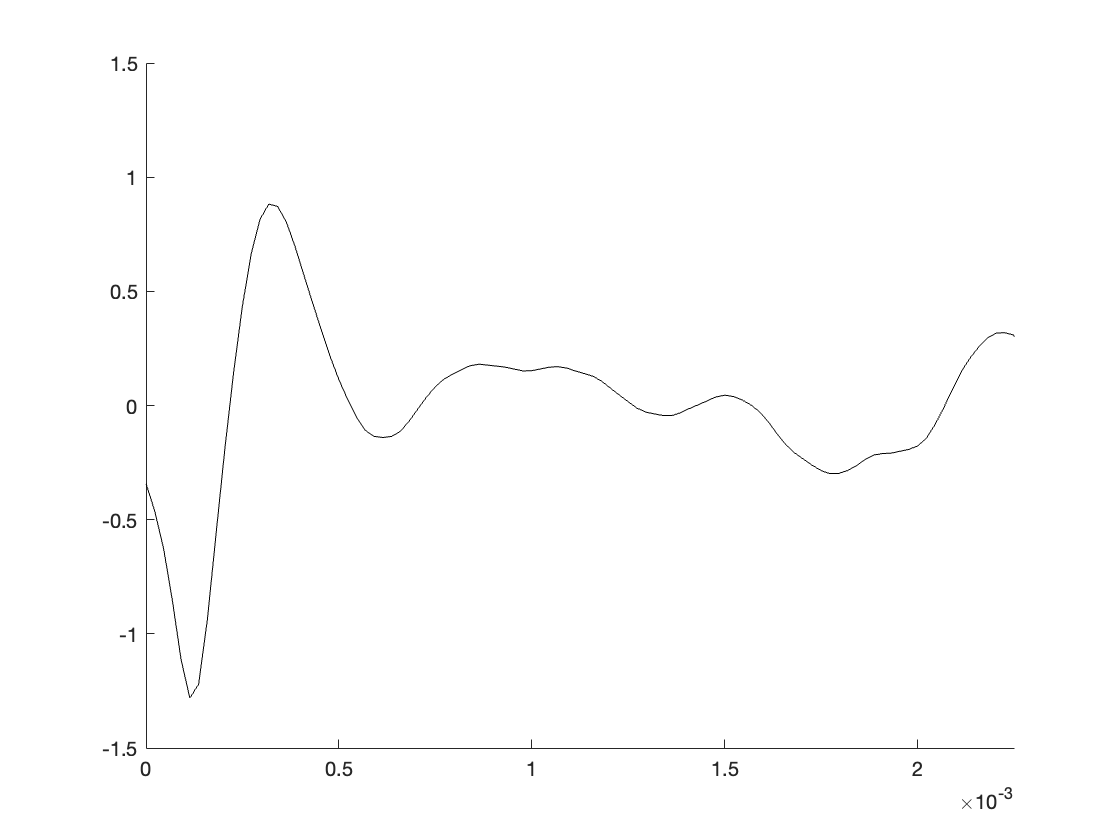
\includegraphics[scale=.16]{trumpetA4_lineplot.png} & 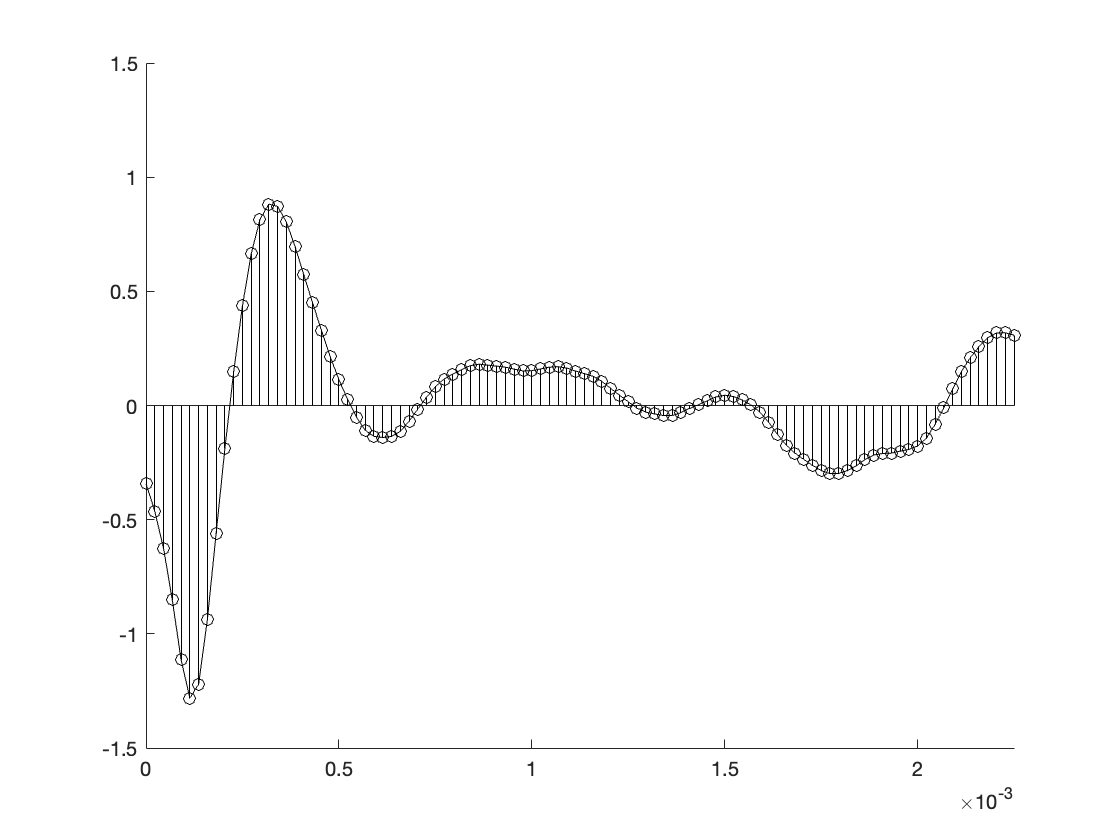
\includegraphics[scale=.16]{trumpetA4_stemplot.png}\\
        The trumpet's unknown waveform $f(t)$ & $f(t)$ sampled 100 times\\
    \end{tabular}
    \caption{Sampling the waveform of a trumpet playing A4}
    \label{fig:trumpetA4_sampled}
\end{figure}

\par \bigskip The first 100 of these samples cover the period of A4's fundamental frequency, $\frac{1}{T} = 440$ Hz. We take those samples as a vector $\mathbf{x}$ and filter it with $100\times 100$ matrices.

\par \bigskip First, we create the frequency response vectors for an LPF and an HPF. We know that the frequencies in $\VNT$ are lowest near the two extremes, $n = 0$ and $n = N$, while frequencies increase as they approach $n = \frac{N}{2}$.\cite{Ryan} To see which frequencies are contributing meaningfully to the tone, we look at the plot of $F_N\mathbf{x}$:

\begin{figure}[h]
    \centering
    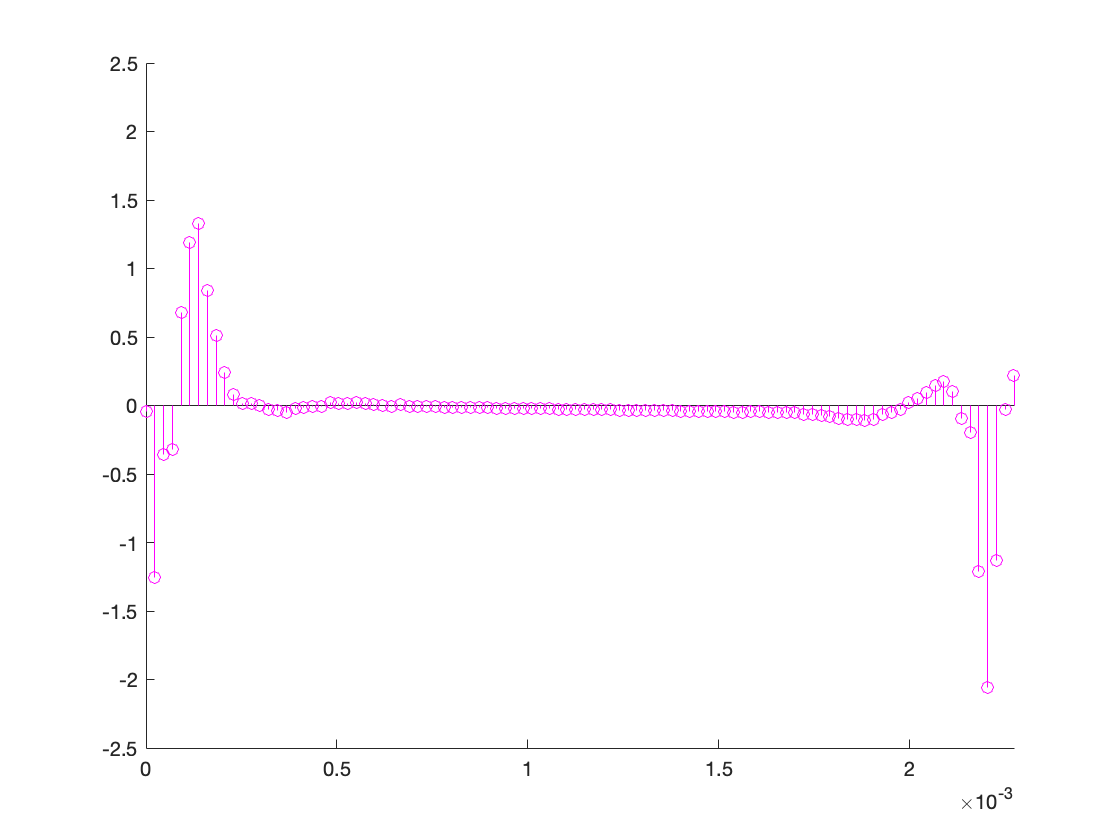
\includegraphics[scale=.16]{DFT_trumpetA4.png}
    \caption{$DFT\mathbf{x}$}
    \label{fig:DFT_trumpetA4}
\end{figure}

\par Seeing that the frequencies become insignificant between $n = 10$ and $n = 90$, we set the frequency responses of the LPF and HPF such that they preserve a similar number of important frequencies:

$$\lambda_{LPF} = \{\underbrace{1,\dots,1}_{5},\underbrace{0,\dots\,0}_{90},\underbrace{1,\dots\,1}_{5}\} \hspace{.5in} \lambda_{HPF} = \{\underbrace{0,\dots,0}_{5},\underbrace{1,\dots\,1}_{90},\underbrace{0,\dots\,0}_{5}\}$$

\par \bigskip Setting $D_{\lambda_{LPF}} = \text{diag}(\lambda_{LPF})$ and $D_{\lambda_{HPF}} = \text{diag}(\lambda_{HPF})$, we obtain $S_{LPF} = F_N^{-1}D_{\lambda_{LPF}}F_N$ and $S_{HPF} = F_N^{-1}D_{\lambda_{HPF}}F_N$. Finally, we can generate two new tones from our sampled trumpet, given by the sample vectors $\mathbf{x}_{LPF} = S_{LPF}\mathbf{x}$ and $\mathbf{x}_{HPF} = S_{HPF}\mathbf{x}$. Figure \ref{fig:trumpetA4_filtered} plots our three vectors over two periods, with their audio realizations linked below.

\par 

\begin{figure}[h]
    \centering
    \begin{tabular}{cc}
        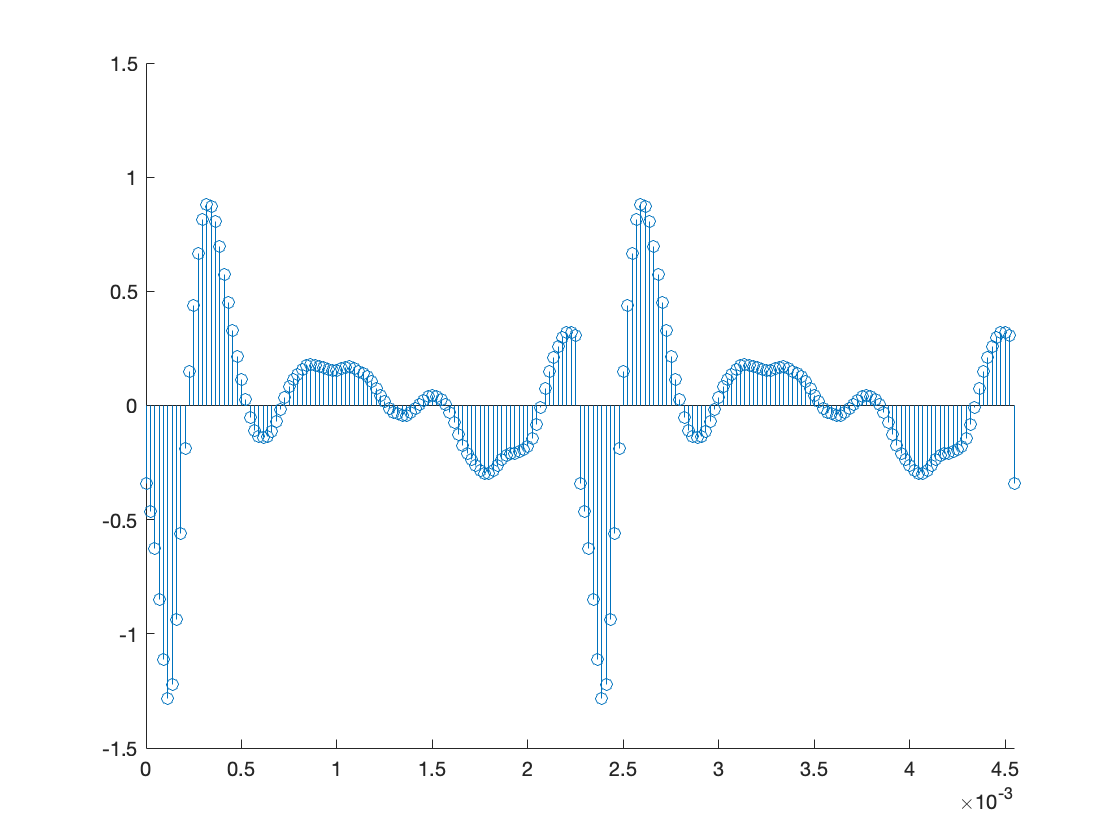
\includegraphics[scale=.18]{trumpetA4.png} & 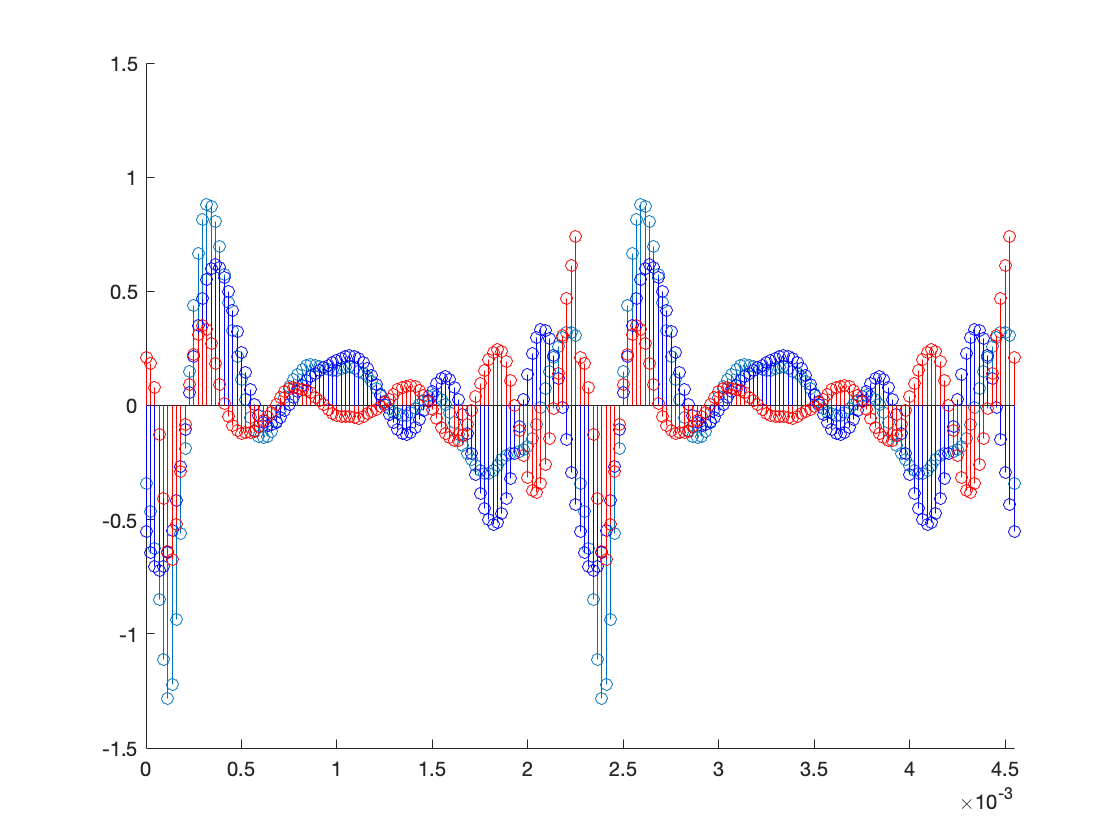
\includegraphics[scale=.18]{trumpetA4_LPF_HPF.png}\\
        \href{https://drive.google.com/file/d/1bsf_KsIPmAkVd0-QYObc78Y2RnRjzCUW/view?usp=sharing}{\color{blue} $[\blacktriangleright]$ $\mathbf{x}$}\\
        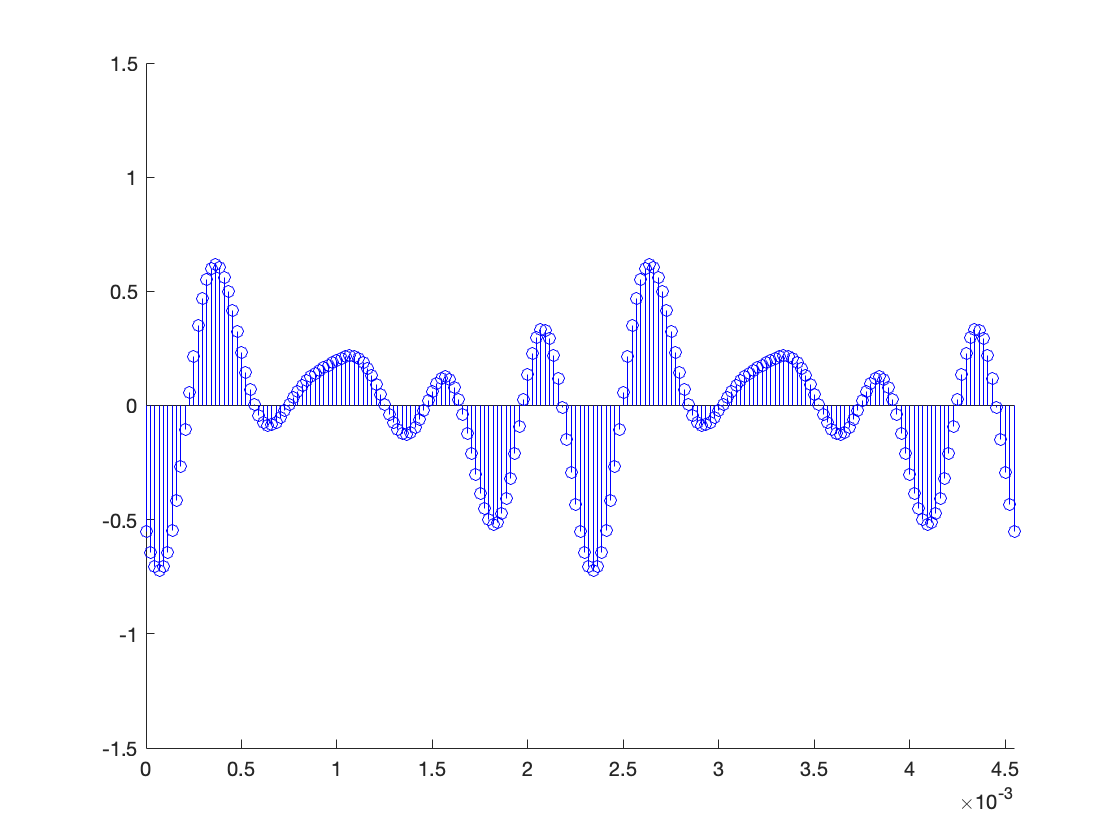
\includegraphics[scale=.18]{trumpetA4_LPF.png} & 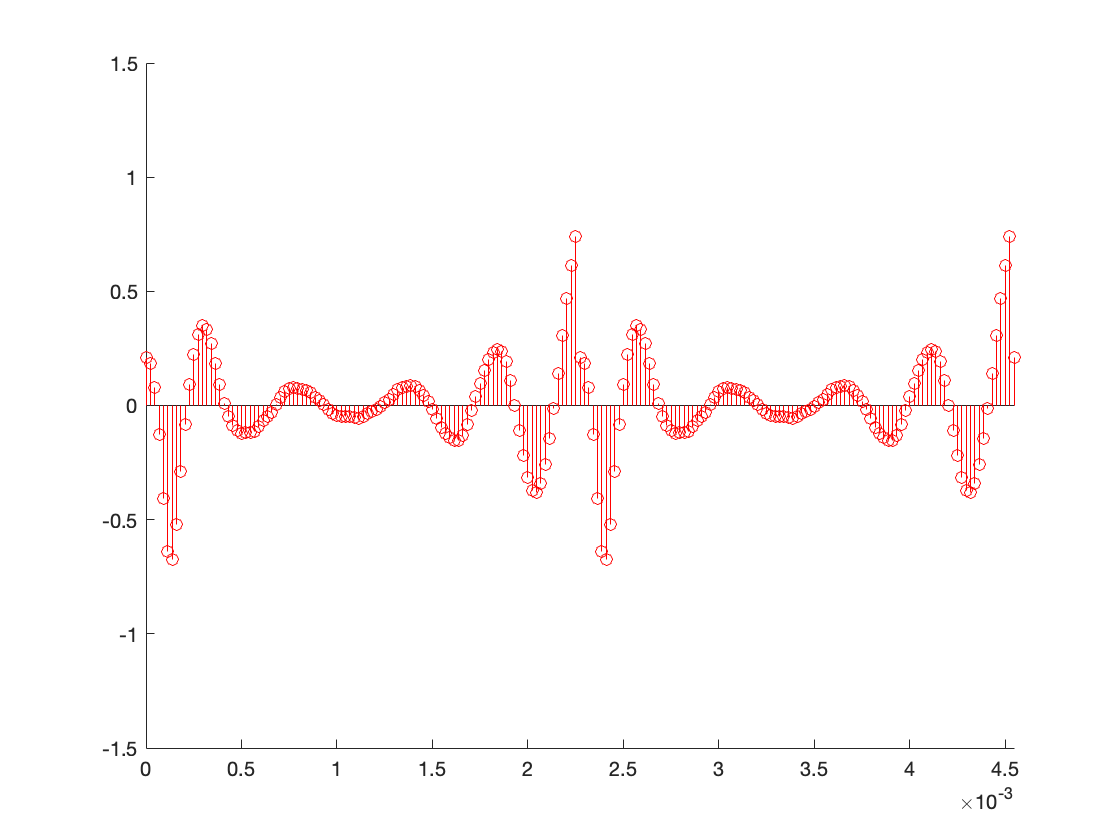
\includegraphics[scale=.18]{trumpetA4_HPF.png}\\
        \href{https://drive.google.com/file/d/11VIUtV8aZl_dNzAf_yXvUNOXUuvRN_Sn/view?usp=sharing}{\color{blue} $[\blacktriangleright]$ $\mathbf{x}_{LPF}$} & \href{https://drive.google.com/file/d/1ZO75jIXYz4RDh-7DFfPc0oz6mco8o-7i/view?usp=sharing}{\color{blue} [$\blacktriangleright$] $\mathbf{x}_{HPF}$}\\
    \end{tabular}
    \caption{Applying the digital LPF and HPF to the trumpet sample}
    \label{fig:trumpetA4_filtered}
\end{figure}

\newpage

\subsection{Conclusion: Tip of The Iceberg}

\par \indentt Digital filters enable music production techniques far beyond manipulating the sound quality of a single sustained note.

\par \bigskip Filters can be applied to an increasing or decreasing degree over time. A series of filters artfully applied to create an effect is called an \textbf{envelope}. Suppose we want to create a ``plucked" note, which quickly decays in amplitude. Then we can simulate a host of instruments which don't sustain notes, such as guitars, pianos, and percussion instruments. By applying a series of low-pass filters over time, we can eliminate frequencies one-by-one from highest to lowest. This replicates how sound decays in the physical world: the higher a frequency, the more quickly it fades away after the vibration that created it has stopped.\cite{Pierce}

\par \bigskip Filters can also be generalized to non-periodic wave functions, opening a whole new can of worms. Such filters operate on irrational vectors called angular frequencies, allowing them to have infinite dimensions. General filters can be applied to any audio clip to smooth the waveform, add reverb and delay, and warp the sound quality of irregular musical sounds like vocals, among many other capabilities.\cite{Ryan}

\par \bigskip Though we must leave much of the world of linear algebra in music unexplored,  hopefully this paper has helped the reader build the necessary confidence to turn knobs like the professionals. For added benefit, the author recommends wearing sunglasses onstage. As a great man once said, ``Let me put my sunglasses on here / So I can see what I'm doing."